% Revisão OK 09/10
\chapter{Plotagem do METAR Histórico}

Para o piloto, é importante ter informações meteorológicas históricas, pois 
essas informações auxiliam na previsão de condições futuras. A meteorologia tende 
a seguir padrões; por exemplo, uma queda na pressão atmosférica geralmente indica 
que as temperaturas podem diminuir posteriormente. Assim, visualizar essas 
informações em gráficos facilita a análise e a tomada de decisões.

Os dados meteorológicos (METARs) coletados de um aeroporto são armazenados na tabela
METAR (vide capítulo de Modelo de Dados) com chave estrangeira ICAO, possibilitando
o armazenamento de múltiplos registros para um único aeródromo. A partir dessa 
tabela, é realizada uma (\textit{query}) que obtém os 12 últimos registros 
de METAR de cada aeródromo. Desse conjunto de dados, usando regex, de forma
semelhante ao Decodificador de Metar, são extraídas seis informações: 
temperatura, ponto de orvalho, velocidade do vento, direção do vento, ajuste altímetro e visibilidade.

Os resultados da consulta são transformados em uma lista de dicionários, onde 
cada dicionário contém essas seis informações.

\begin{verbatim}
    metar_data = [
        {
            "temperature": 20 ,
            "dew_point": 15,
            "wind_speed": 12,
            "wind_direction": 120,
            "qnh": 1030,
            "visibility": 9999,
        },
        {
            "temperature": 21 ,
            "dew_point": 13,
            "wind_speed": 5,
            "wind_direction": 129,
            "qnh": 1028,
            "visibility": 9999,
        },
        ...
    ]
\end{verbatim}


Essa lista é então passada para a biblioteca \texttt{matplotlib}, que gera três 
gráficos em um estilo personalizado para combinar com o tema escuro da página. 
Cada gráfico combina duas informações. Temos dois eixos Y e eixo X compartilhado.
Os gráficos são salvos como SVG na pasta de arquivos estáticos.

As imagens de plot seguem um padrão, o código ICAO do aeroporto e os dados 
específicos são utilizados na geração do nome do arquivo SVG ("icao-dado1-dado2.svg"). 
Ao carregar a página, as imagens são exibidas diretamente por meio de tags \texttt{<img>},
 que apontam para os gráficos salvos na pasta estática.

Como na consulta do METAR, esta tarefa é realizada assincronamente nos 
minutos 0, 20, 40 (vide capítulo de arquitetura). Então, quando o usuário carrega a 
página, as plotagens já encontram-se prontas segindo o segundo princípio norteador.

\begin{figure}[ht]
    \begin{center}
    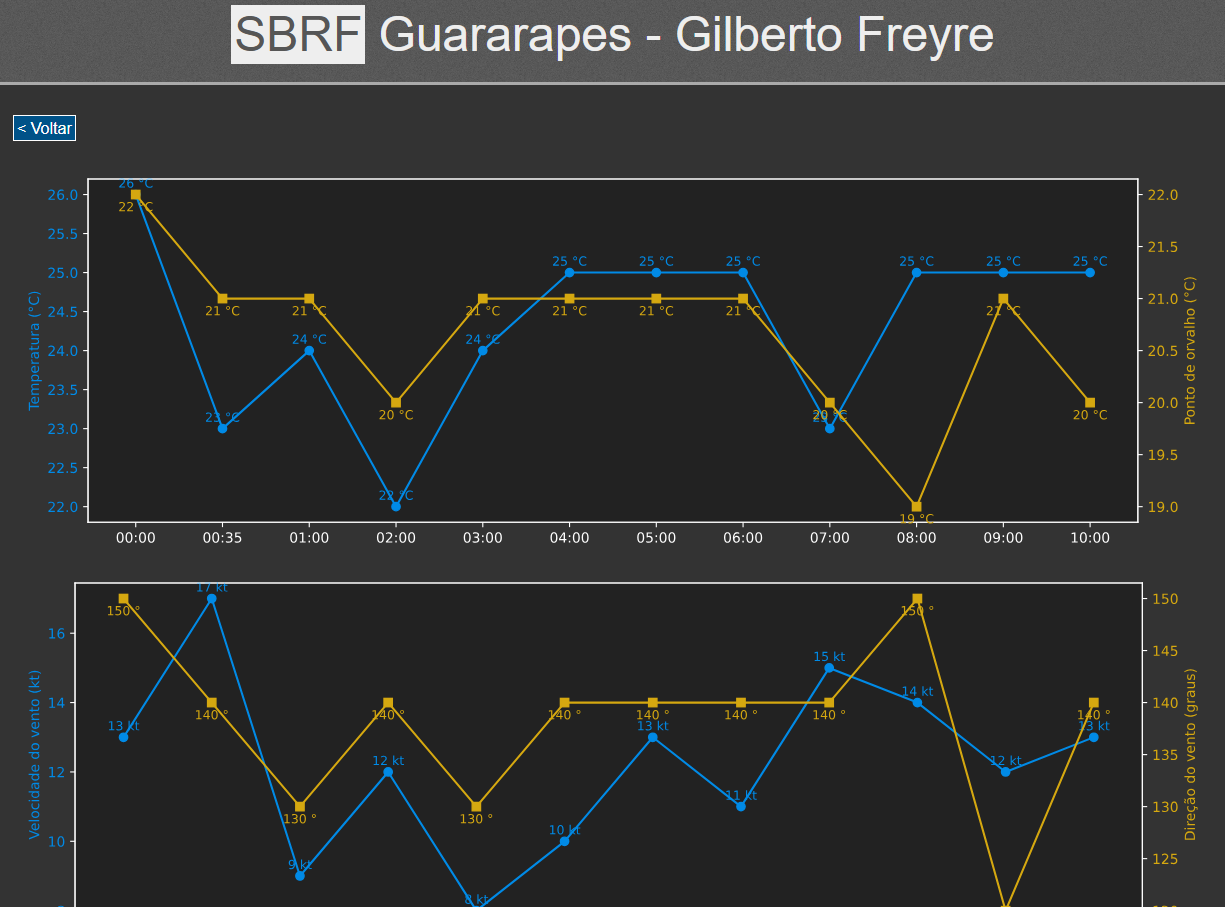
\includegraphics[width=400pt]{img/plots-SBRF.png}
    \caption{Gráficos do aeroporto Aeroporto Internacional do Recife do dia 28 de agosto de 2024}
    \label{fig:sbrf-plot}
    \end{center}
\end{figure}